\documentclass[a4paper,10pt]{article}
\input{/Users/benjamin/Documents/Education/LaTeX/macro.tex}

\title{COA: S�ance 1}
\author{Benjamin \bsc{Van Ryseghem}}

\begin{document}
\maketitle

\section{Exercice 1: Phase d'analyse des besoins d'une r�servation de chambre d'h�tel}
\begin{tabular}{|c|c|c|}
\hline
Concept & Type (class/actor/UC) & Definition \\
\hline
\hline
R�ceptionniste & actor & \\
R�server une chambre & UC & \\
Client & class & \\
Directeur & actor & \\
Lister les chambres & UC & \\
Syst�me & actor & Administrateur \\
G�rer les chambres & UC & \\
Hotel & class & \\
Chambre & class & \\
Salle d'eau & class & \\
Douche & class & \\
Salle de bain & class & \\
�tablir une facture & UC & \\
\hline
\end{tabular}

\begin{figure}[ht]
\begin{center}
     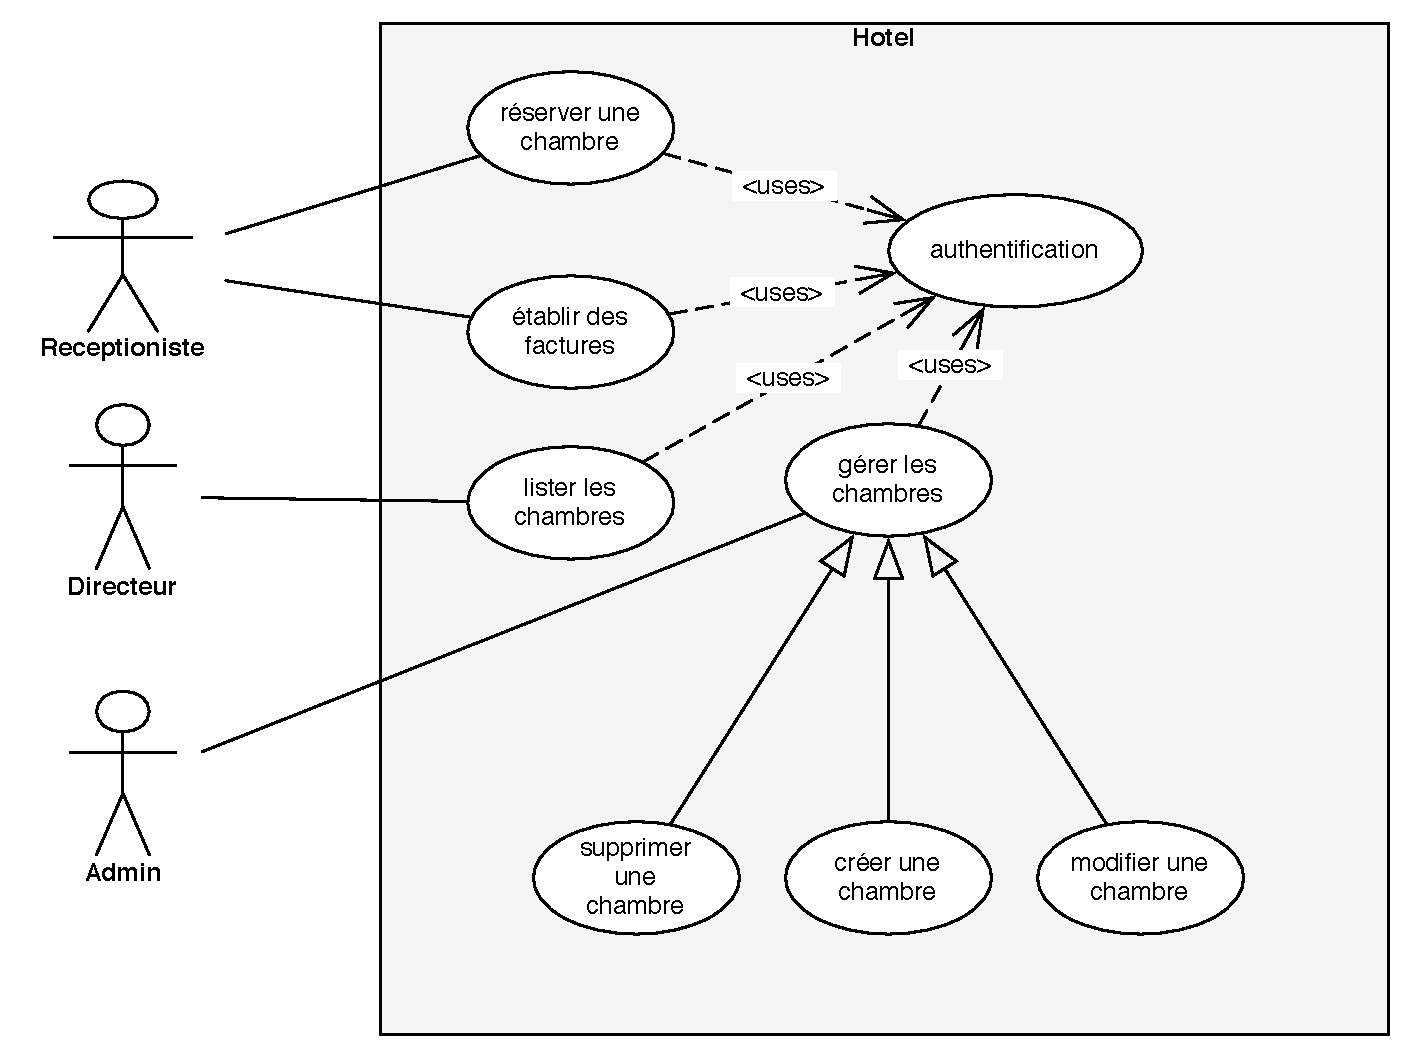
\includegraphics[width=15cm]{figures/Diagramme_CU.pdf}
\end{center}
     \caption{Diagramme des cas d'utilisation}
\end{figure}

\begin{figure}[ht]
\begin{center}
     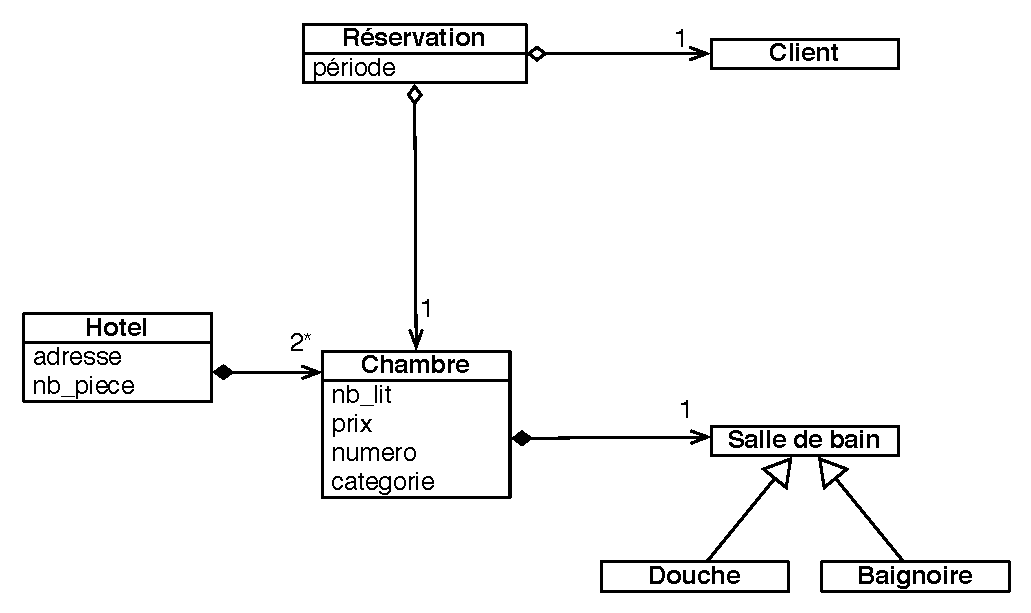
\includegraphics[width=15cm]{figures/Diagramme_Classes.pdf}
\end{center}
     \caption{Diagramme de Classes}
\end{figure}

\signature

\end{document}